\chapter{Kinematics}

How can we describe the motion of objects other than falling bodies? Kinematics 
is the description of motion. 

%intro explaining usefulness of kinematics
%derive kinematics eqs from concrete examples


\begin{mdframed}[style=important]
\begin{equation}
    x_f = x_0 + v_0 t + \frac{1}{2}at^2
\end{equation}
\begin{equation}
    v_f = v_0 + at
\end{equation}
\begin{equation}
    x_f = x_0 + \frac{1}{2}\left(v_f + v_0 \right)t
\end{equation}
\begin{equation}
    v_f^2 = v_0^2 + 2a\left(x_f - x_0 \right)
\end{equation}

\begin{equation}
    \Delta x - x_0 = v_{\text{avg}}t
\end{equation}
Note that $v_0$ and $v_i$ are synonomous, some professors will use $v_0$ to mean ``velocity not`` or inital velocity.
%FIXME expand, write what all variables mean
\end{mdframed}




Note that each equation is missing a certain variable (or two)
\begin{itemize}
    \item (5.1) is missing $v_f$. 
    \item (5.2) is missing $x_i$ or $x_f$
    \item (5.3) is missing $a$
    \item (5.4) is missing $t$
    \item (5.5) is missing $a$
\end{itemize} 

It is important to note that these equations only work when the acceleration is held constant, which is referred to as \newterm{uniformly accelerated motion}. 

\textbf{Example}: Terri and Jerry are running a race. Terri has a maximum 
acceleration of 3.4 $m/s^2$ and a top speed of 9.2 $m/s$. Jerry has a maximum 
acceleration of 3.7 $m/s^2$ and a top speed of 8.7 $m/s$. If the race is 200 $m$ 
long, who will win? Assume that each runner has maximum acceleration until they 
reach their top speed and that they will maintain that top speed once they reach 
it. 

\textbf{Solution}: We want to know how long it takes each runner to complete the 
200 $m$ race. For each runner, we will divide their run into two sections:
\begin{enumerate}
\item The time they are accelerating to their top speed
\item The time they are maintaining their top speed
\end{enumerate}

We can use a table to track the results of our calculations:
\begin{center}
\begin{tabular}{|c|c|c|}
\hline
Runner & Terri & Jerry\\\hline
Leg 1 (s) & & \\\hline
Leg 2 (s) & & \\\hline
Total (s) & & \\\hline
\end{tabular}
\end{center}

We'll begin with Terri's first leg. Taking the starting line as $x = 0$, we know 
that:
$$x_0 = 0\text{ }m$$
$$v_0 = 0\text { } \frac{m}{s}$$
$$a = 3.4\text{ }\frac{m}{s^2}$$

And since we want to know how long it takes Terri to reach her top speed, we 
also know that $v_f = 9.2$ $m/s$. Since we don't know how far Terri will run 
before she reaches her top speed (and we're not looking for that quantity), we 
need to select an equation that does not include $x$:
$$v_f = v_0 + at$$
$$9.2 \frac{m}{s} = 0 \frac{m}{s} + \left(3.4 \frac{m}{s^2} \right)t$$
$$t = \frac{9.2 \frac{m}{s}}{3.4 \frac{m}{s^2}} \approx 2.7\text{ }s$$

With a similar method, we can find how long it takes Jerry to reach his top 
speed:
$$t = \frac{v_f}{a} = \frac{8.7 \frac{m}{s}}{3.7 \frac{m}{s^2}} \approx 2.4
\text{ }s$$

Let's go ahead and record this in our table:
\begin{center}
\begin{tabular}{|c|c|c|}
\hline
Runner & Terri & Jerry\\\hline
Leg 1 (s) & 2.7 & 2.4 \\\hline
Leg 2 (s) & & \\\hline
Total (s) & & \\\hline
\end{tabular}
\end{center}

Now that we know how much time it takes each runner to reach their top speed, we 
need to figure out how much time it takes them to complete the race from the 
point at which each reaches their top speed. To do this, we will first have to 
find \textit{where} each runner hits their top speed. (This is because we can't 
use $v_f = v_0 + at$ to find a time anymore, since from now on the runners' 
accelerations are zero, and all the other equations involve $x$.) For each 
runner, we know $a$, $v_0$, $v_f$, $x_0$, and $t$. You could choose any equation, 
but we will use this one:
$$x_f = x_0 + \frac{1}{2} \left( v_f + v_0 \right)t$$

Since each runner begins on the starting line, $x_0 = 0$ $m$ and $v_0 = 0$ $m/s$:
$$x_f = \frac{v_f \cdot t}{2}$$

For Terri:
$$x_f = \frac{\left(9.2 \frac{m}{s} \right) \left(2.7\text{ }s \right)}{2} 
\approx 12.4 \text{ }m$$

For Jerry:
$$x_f = \frac{\left( 8.7 \frac{m}{s} \right) \left( 2.4 \text{ }s \right)}{2} 
\approx 10.2 \text{ }m$$

Now that we know where they reach their top speed, we can take that position as 
$x_0$ and find how long it takes each runner to reach the finish line at $x_f = 
200\text{ }m$. Since $a = 0$ $m/s^2$, we can use:
$$x_f = x_0 + v_0 t$$

Rearranging to solve for $t$:
$$t = \frac{x_f - x_0}{v_0}$$

For Terri:
$$t = \frac{200 \text{ } m - 12.4 \text{ } m}{9.2 \text{ } \frac{m}{s}} \approx 
20.4\text{ }s$$

And for Jerry:
$$t = \frac{200 \text{ } m - 10.2 \text{ } m}{8.7 \text{ } \frac{m}{s}} \approx 
21.8 \text{ } s$$

Completing our table, we see that Terri will win the race by finishing in the 
least amount of time:
\begin{center}
\begin{tabular}{|c|c|c|}
\hline
Runner & Terri & Jerry\\\hline
Leg 1 (s) & 2.7 & 2.4 \\\hline
Leg 2 (s) & 20.4 & 21.8 \\\hline
Total (s) & 23.1 & 24.2 \\\hline
\end{tabular}
\end{center}

\section{Graphing Motion}

\subsection{Motion Diagrams}
%explanation of constnat time interval motion diagrams

\textbf{Example}: Create a motion diagram of a ball rolling with a constant 
acceleration down an incline (the acceleration is in the same direction as 
motion). 

\textbf{Solution}: The ball is accelerating down the ramp, so it will cover 
more distance each second. You could draw your ramp going left or right, as 
long as the distance covered each time interval increases as time passes. 

\begin{center}
 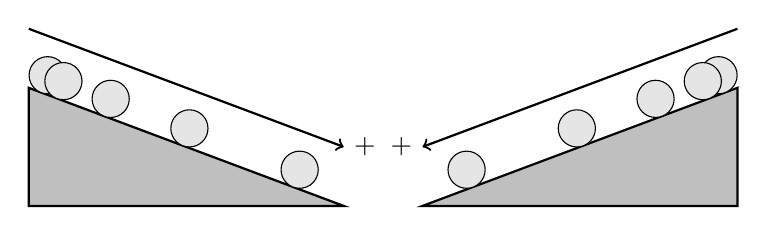
\begin{tikzpicture}
    %left ramp
    \draw[thick, fill=gray!50] (0.5,0.5) -- (4.5, 0.5) -- (0.5, 2) -- cycle;
    \foreach \t in {0, 1, 4, 9, 16}
        \draw[fill=gray!20] (0.74+0.2*\t, 2.16-0.075*\t) circle (0.236cm);
    \draw[->, thick] (0.5, 2.75) -- (4.5, 1.25) node[right] {+};
    
    %right ramp
    \draw[thick, fill=gray!50] (5.5, 0.5) -- (9.5, 0.5) -- (9.5, 2) -- cycle;
    \foreach \t in {0, 1, 4, 9, 16}
        \draw[fill=gray!20] (9.26-0.2*\t, 2.16-0.075*\t) circle (0.236cm);
    \draw[->, thick] (9.5, 2.75) -- (5.5, 1.25) node[left] {+};  
\end{tikzpicture}   
\end{center}

\subsection{Position-Time and Velocity-Time Graphs}

%interpretation of x-t and v-t graphs without explicit calculus

In the example problem above, graphs of each runner's motion would allow us to 
immediately see who would win. We can describe Terri's and Jerry's runs with 
piecewise functions:
$$x_{Terri}(t) = \begin{cases}
\left( 1.7 \text{ } \frac{m}{s^2} \right)t^2 & \text{if } 0 \leq t < 2.7 
\text{ }s\\
12.4 \text{ } m + \left( 9.2 \text{ } \frac{m}{s} \right) \left( t - 2.7 \text{ } 
s \right) & \text{if } t \geq 2.7 \text{ }s
\end{cases}$$

$$x_{Jerry}(t) = \begin{cases}
\left( 1.85 \text{ } \frac{m}{s^2} \right)t^2 & \text{if } 0 \leq t < 2.4 
\text{ }s\\
10.2 \text{ }m + \left( 8.7 \text{ }\frac{m}{s} \right) \left(t - 2.4 \text{ }s 
\right) & \text{if } t \geq 2.4 \text{ }s
\end{cases}$$

Graphing Terri in red and Jerry in blue:
\begin{center}
    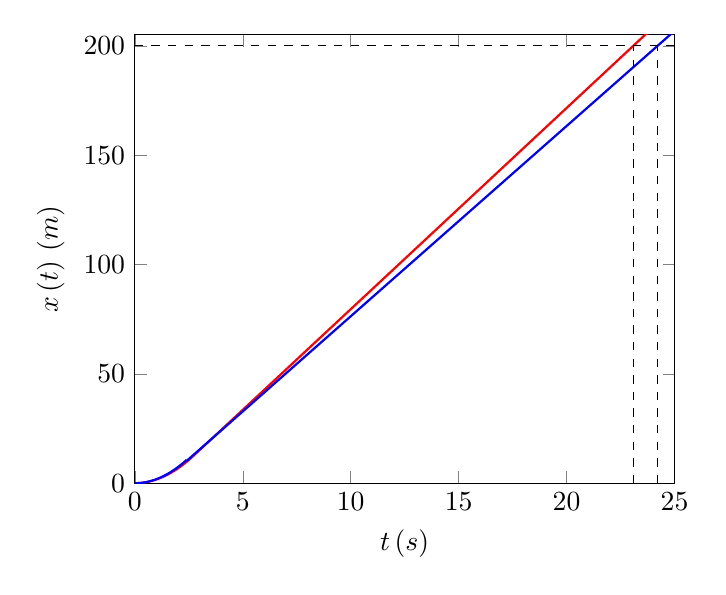
\begin{tikzpicture}
        \begin{axis}[xmin = 0, ymin = 0, xmax = 25, ymax = 205, xlabel = {$t\text{ }
        \left(s \right)$}, ylabel = {$x \left( t \right)\text{ }\left( m \right)$}]
            \addplot[red, thick, domain = 0:2.7] {1.7*x^2};
            \addplot[red, thick, domain = 2.7:25] {12.4 + 9.2*(x-2.7)};
            \addplot[blue, thick, domain = 0:2.4] {1.85*x^2};
            \addplot[blue, thick, domain = 2.4:25] {10.2 + 8.7*(x-2.4)};
            \addplot[dashed, domain = 0:25] {200};
            \draw[dashed] (23.1, 0) -- (23.1, 200);
            \draw[dashed] (24.2, 0) -- (24.2, 200);
        \end{axis}
    \end{tikzpicture}
\end{center}

Since the red function (Terri) crosses $x(t) = 200 \text{ }m$ first, we see that 
Terri will win. 

\begin{Exercise}[label = graphs]
The following graphs show the position of an object from $t = 0\text{ }s$ to 
$t = 10\text{ }s$. The scales on the $y$-axes are all the same. 

\begin{center}
 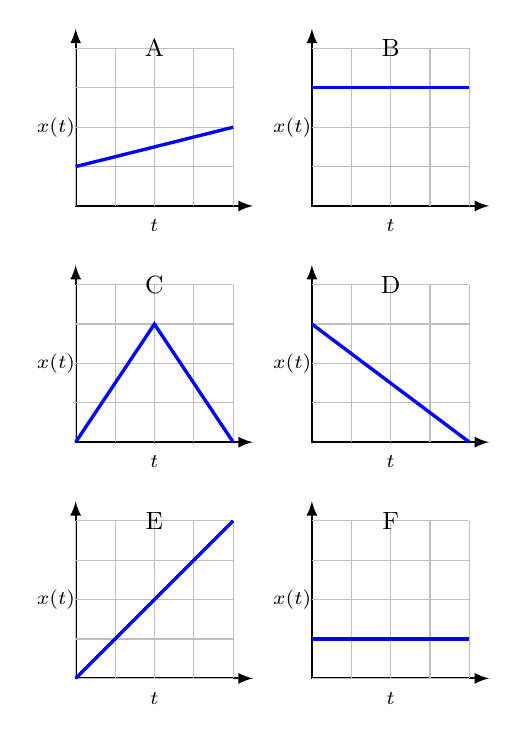
\begin{tikzpicture}
    %graph A
    \draw[thick, latex-latex] (0.5, 8.75) -- (0.5, 6.5) -- (2.75, 6.5);
    \draw[gray!50, step = 0.5cm] (0.5, 6.5) grid (2.5, 8.5);
    \node[font = \scriptsize] at (1.5, 6.25) {$t$};
    \node[font = \scriptsize] at (0.25, 7.5) {$x(t)$};
    \draw[blue, very thick] (0.5, 7) -- (2.5, 7.5);
    \node[font = \small] at (1.5, 8.5) {A};

    %graph B
    \draw[thick, latex-latex] (3.5, 8.75) -- (3.5, 6.5) -- (5.75, 6.5);
    \draw[gray!50, step = 0.5cm] (3.5, 6.5) grid (5.5, 8.5);
    \node[font = \scriptsize] at (4.5, 6.25) {$t$};
    \node[font = \scriptsize] at (3.25, 7.5) {$x(t)$};
    \draw[blue, very thick] (3.5, 8) -- (5.5, 8);
    \node[font = \small] at (4.5, 8.5) {B};
    
    %graph C
    \draw[thick, latex-latex] (0.5, 5.75) -- (0.5, 3.5) -- (2.75, 3.5);
    \draw[gray!50, step = 0.5cm] (0.5, 3.5) grid (2.5, 5.5);
    \node[font = \scriptsize] at (1.5, 3.25) {$t$};
    \node[font = \scriptsize] at (0.25, 4.5) {$x(t)$};
    \draw[blue, very thick] (0.5, 3.5) -- (1.5, 5) -- (2.5, 3.5);
    \node[font = \small] at (1.5, 5.5) {C};

    %graph D
    \draw[thick, latex-latex] (3.5, 5.75) -- (3.5, 3.5) -- (5.75, 3.5);
    \draw[gray!50, step = 0.5cm] (3.5, 3.5) grid (5.5, 5.5);
    \node[font = \scriptsize] at (4.5, 3.25) {$t$};
    \node[font = \scriptsize] at (3.25, 4.5) {$x(t)$};
    \draw[blue, very thick] (3.5, 5) -- (5.5, 3.5);
    \node[font = \small] at (4.5, 5.5) {D};

    %graph E
    \draw[thick, latex-latex] (0.5, 2.75) -- (0.5, 0.5) -- (2.75, 0.5);
    \draw[gray!50, step = 0.5cm] (0.5, 0.5) grid (2.5, 2.5);
    \node[font = \scriptsize] at (1.5, 0.25) {$t$};
    \node[font = \scriptsize] at (0.25, 1.5) {$x(t)$};
    \draw[blue, very thick] (0.5, 0.5) -- (2.5, 2.5);
    \node[font = \small] at (1.5, 2.5) {E};

    %graph F
    \draw[thick, latex-latex] (3.5, 2.75) -- (3.5, 0.5) -- (5.75, 0.5);
    \draw[gray!50, step = 0.5cm] (3.5, 0.5) grid (5.5, 2.5);
    \node[font = \scriptsize] at (4.5, 0.25) {$t$};
    \node[font = \scriptsize] at (3.25, 1.5) {$x(t)$};
    \draw[blue, very thick] (3.5, 1) -- (5.5, 1);
    \node[font = \small] at (4.5, 2.5) {F};
\end{tikzpicture}   
\end{center}


Rank the objects from least to greatest (all negative values are lower than 
all positive values) in terms of:
\begin{enumerate}
    \item displacement from $t = 0\text{ }s$ to $t = 10\text{ }s$.
    \item instantaneous velocity at $t = 7.5\text{ }s$.
    \item distance traveled from $t = 0\text{ }s$ to $t = 10\text{ }s$
\end{enumerate}
\end{Exercise}

\begin{Answer}[ref = graphs]
\begin{enumerate}
	\item D, B/C/F, A, E; displacement is the difference in position between the 
	starting and ending points. Object D moves backwards and therefore has a 
	negative displacement. Objects B, C, and F all end in the same position they 
	started and therefore have zero displacement. Objects A and E both move 
	forward and have positive displacement. Object E moves forward 4 units while 
	Object A only moves forward by 1 unit. Therefore, object E has a greater 
	positive displacement than object A.  
	\item C, D, B/F, A, E; instantaneous velocity is given by the slope of a 
	position-time graph at the indicated time (in this case, $t = 7.5s$). Since 
	the graphs show 10 seconds of motion and there are 4 tick marks on each 
	$x$-axis, each unit on the $x$-axis represents 2.5 seconds of time. Therefore, 
	$t = 7.5s$ is the third tick mark on the $x$-axis. At $t = 7.5s$, the graphs of 
	objects C and D have negative slopes and therefore negative velocities. Since 
	the slope for object C is steeper than the slope for object D, object C's 
	\textit{speed} is greater than object D's, and object C's \textit{velocity} 
	is more negative than object D's. The graphs of object's B and F are horizontal 
	at $t=7.5s$ and therefore their velocities are zero. Graphs A and E have 
	positive slopes, and since E is steeper, object E has a greater speed and 
	more positive velocity than object A. 
	\item B/F, A, D, E, C; distance is a scalar and therefore always positive. B 
	and F do not change position, and therefore travel a distance of 0. A moves 
	forward 1 unit. D moves backwards 3 units (for a \textit{distance} of 3). E 
	moves forward 4 units. C moves forwards 3 units, then backwards 3 additional 
	units, for a total of 6 units of distance. 
\end{enumerate}
\end{Answer}


\section{Separation of Components}
In the current chapter, we have learned how to use kinematics to describe 
one-dimensional motion. In the next chapter, you will learn to describe 
two-dimensional motion. It turns out that you can treat the different dimensions 
(horizontal and vertical motion) separately! Consider this scenario: A cannonball 
is shot from a cliff and the same instant an identical cannonball is dropped from 
the same cliff (see...). If the cannon is aimed horizontally, which cannonball 
will hit the ground first?

%FIXME image of cannon example

Go ahead and jot down what you think would happen: would the dropped ball hit 
first, the launched ball hit first, or would they both reach the ground below at 
the same time? Then, take a look at this video: 
\url{https://www.youtube.com/watch?v=zMF4CD7i3hg}. In it, two balls are released 
from the same height at the same time. One is dropped from rest while the other 
is launched horizontally (that is, its initial velocity is entirely in the 
$x$-direction). Based on the video, was your cannonball prediction correct? 
We'll learn to explain this phenomenon in the next chapter. 